% !TeX root = main.tex

\chapter{Matrix Multiplication}
\glsresetall
\label{chapter:matrix_multiplication}

This chapter looks at a bit more complex design -- matrix multiplication. We consider two different versions. We start with a ``straightforward'' implementation, i.e., one that takes two matrices as inputs and outputs the result of their multiplication. We call this complete matrix multiplication. Then, we look at a block matrix multiplication. Here the input matrices are feed into the function in portions, and the function computes partial results.

\section{Background}

Matrix multiplication is a binary operation that combines two matrices into a third. The operation itself can be described as a linear operation on the vectors that compose the two matrices. The most common form of matrix multiplication is call the \term{matrix product}. The matrix product $\mathbf{AB}$ creates an $n \times p$ matrix when matrix $\mathbf{A}$ has dimensions $n \times m$ and matrix $\mathbf{B}$ has dimensions $m \times p$. 

More precisely, we define the following: \begin{equation}
\mathbf{A} =
 \begin{bmatrix}
  A_{11} & A_{12}  & \cdots & A_{1m} \\
  A_{21} & A_{22}  & \cdots & A_{2m} \\
  \vdots  & \vdots  &\ddots & \vdots  \\
    A_{n1} & A_{n2}  & \cdots & A_{nm} \\
 \end{bmatrix},  \quad
\mathbf{B} =
 \begin{bmatrix}
  B_{11} & B_{12}  & \cdots & B_{1p} \\
  B_{21} & B_{22}  & \cdots & B_{2p} \\
  \vdots  & \vdots   &\ddots & \vdots  \\
  B_{m1} & B_{m2}  & \cdots & B_{mp} \\
 \end{bmatrix}
\end{equation} 

\begin{equation}
\mathbf{AB} = \begin{bmatrix}
 \left(\mathbf{AB}\right)_{11} & \left(\mathbf{AB}\right)_{12} & \cdots & \left(\mathbf{AB}\right)_{1p} \\
 \left(\mathbf{AB}\right)_{21} & \left(\mathbf{AB}\right)_{22} & \cdots & \left(\mathbf{AB}\right)_{2p} \\
\vdots & \vdots & \ddots & \vdots \\
 \left(\mathbf{AB}\right)_{n1} & \left(\mathbf{AB}\right)_{n2} & \cdots & \left(\mathbf{AB}\right)_{np} \\
\end{bmatrix}
\end{equation} where the operation $\left(\mathbf{AB}\right)_{ij}$ is defined as $\left(\mathbf{A}\mathbf{B}\right)_{ij} = \sum_{k=1}^m A_{ik}B_{kj}$.

Now we provide a simple example. Let
\begin{equation}
\mathbf{A} =
 \begin{bmatrix}
 \label{eq:ABmatrix}
  A_{11} & A_{12}  &  A_{13} \\
  A_{21} & A_{22} & A_{23} \\
 \end{bmatrix},  \quad
\mathbf{B} =
 \begin{bmatrix}
  B_{11} & B_{12}  \\
  B_{21} & B_{22}   \\
   B_{31} & B_{32}  \\
 \end{bmatrix}
\end{equation}
The result of the matrix product is
\begin{equation}\label{eq:ABmatrix_product}\mathbf{AB} = \begin{bmatrix}
 A_{11}B_{11} + A_{12}B_{21} + A_{13}B_{31} & A_{11}B_{12} + A_{12}B_{22} + A_{13}B_{32} \\
 A_{21}B_{11} + A_{22}B_{21} + A_{23}B_{31} & A_{21}B_{12} + A_{22}B_{22} + A_{23}B_{32}\\
\end{bmatrix}
\end{equation}

Matrix multiplication is a fundamental operation in numerical algorithms. Computing the product between large matrices can take a significant amount of time. Therefore, it is critically important part of many of problems in numerical computing. Fundamentally, matrices represent linear transforms between vector spaces; matrix multiplication provides way to compose the linear transforms.  Applications include linearly changing coordinates (e.g., translation, rotation in graphics), high dimensional problems in statistical physics (e.g., transfer-matrix method), and graph operations (e.g., determining if a path exists from one vertex to another). Thus it is a well studied problem, and there are many algorithms that aim to increase its performance, and reduce the memory usage.

\begin{figure}
\lstinputlisting[firstline=5]{examples/matrixmultiplication.cpp}
\caption{A common three \lstinline{for} loop structure for matrix multiplication. The outer \lstinline{for} loops, labeled \lstinline{rows} and \lstinline{cols}, iterate across the rows and columns of the output matrix $\mathbf{AB}$.  The innermost loop, labeled \lstinline{product} multiplies the appropriate elements of one row of $\mathbf{A}$ and one column of $\mathbf{B}$ and accumulates them until it has the result for the element in $\mathbf{AB}$ .  }
\label{fig:matrixmultiplication_sw}
\end{figure}

\section{Complete Matrix Multiplication}

We start our optimization process with perhaps the most common method to compute a matrix multiplication -- using three nested \lstinline{for} loops. Figure \ref{fig:matrixmultiplication_sw} provides the code for such an implementation.  The outer \lstinline{for} loops, labeled \lstinline{rows} and \lstinline{cols}, iterate across the rows and columns of the output matrix $\mathbf{AB}$. The innermost \lstinline{for} loop computes a dot product of one row of $\mathbf{A}$ and one column of $\mathbf{B}$. Each dot product is a completely independent set of computations that results in one element of $\mathbf{AB}$.  Conceptually, we are performing \lstinline{P} matrix-vector multiplications, one for each column of $\mathbf{B}$.

In this case, we've applied a \lstinline{pipeline} directive to the \lstinline{col} loop with a target initiation interval of 1. The result is that the innermost \lstinline{for} loop is fully unrolled, and we expect the resulting circuit include roughly $M$ multiply-add operators and to have an interval of roughly $N*P$ cycles.  As discussed in Chapter \ref{chapter:dft}, this is only one reasonable choice.  We could choose to place the \lstinline{pipeline} directive in different locations in the function with the goal of achieving different resource-throughput tradeoffs. For instance, placing the same directive at the top of the function (outside all of the \lstinline{for} loops) will result in all of the loops being completely unrolled, which would take roughly $N*M*P$ multiply-add operators and would have an interval of 1 cycle. Placing it inside the \lstinline{row} loop would result in roughly $M*P$ multiply-add operators and an interval of roughly $N$ cycles. These design points are relatively easy to achieve, given the corresponding array partitioning.  It's also possible to pipeline the innermost loop with the goal of achieving a design with only one multiply-add operator, although achieving an II=1 implementation at high clock frequencies can be difficult because of the recurrence involved in the accumulation of variable \lstinline{ABij}.  We can also partially unroll different loops to achieve yet more design points.  The fundamental tradeoff here is between the complexity of the resulting architecture, i.e., the number of multiply-add operators, and performance, i.e., the number of cycles that the hardware is busy.  In an ideal world, each doubling of the resource usage should result in exactly half the number of clock cycles being required, although in practice such `perfect scaling' is difficult to achieve.

\begin{exercise}
Change the location of the \lstinline{pipeline} directive. How does the location effect the resource usage? How does it change the performance? Which alternative provides the best performance in terms of function interval? Which provides the smallest resource usage? Where do you think is the best place for the directive? Would increasing the size of the matrices change your decision?
\end{exercise}

Executing large numbers of operations every cycle requires being able to supply all of the required operands and to store the results of each operation.   Previously we have used the \lstinline{array_partition} directive to increase the number of accesses that can be performed on each memory.  As long as the partition of the array that each memory access can be determined at compile time, then array partitioning is a simple and efficient way to increase the number of memory accesses that can be performed each clock cycle.  In this case, we use the slightly different \lstinline{array_reshape} directive to perform array partitioning.  This directive not only partitions the address space of the memory into separate memory blocks, but then recombines the memory blocks into a single memory.  This transformation increases the data width of the memory used to store the array, but doesn't change the overall number of bits being stored.  The difference is shown in Figure \ref{fig:matmul_array_reshape}.

\begin{figure}
\centering
\includesvg{matmul_array_reshape}
\caption{Three different implementations of a two-dimensional array.  On the left is the original array consisting of $N*M$ elements.  In the middle, the array has been transformed using the \lstinline{array_partition} directive, resulting in $M$ memories, each with $N$ elements.  On the right, the array has been transformed using the \lstinline{array_reshape} directive, resulting in one memory with $N$ locations and each location contains $M$ elements of the original array.}
\label{fig:matmul_array_reshape}
\end{figure}

Both \lstinline{array_reshape} and \lstinline{array_partition} increase the number of array elements that can be read each clock cycle.  They also support the same options, enabling \lstinline{cyclic} and \lstinline{block} partitions or partitioning along different dimensions of a multi-dimensional array.  In the case of \lstinline{array_reshape}, the elements must each have the same address in the transformed array, whereas with \lstinline{array_partition}, the addresses in the transformed array can be unrelated.  Although it may seem like one would always want to use \lstinline{array_partition} because it is more flexible, it makes each individual memory smaller, which can sometimes result in inefficient memory usage.  The \lstinline{array_reshape} directive results in larger memory blocks, which can sometimes be mapped more efficiently into primitive FPGA resources.   In particular, the smallest granularity of \gls{bram} blocks in Xilinx Virtex Ultrascale+ devices is 18 Kbits with several different supported combination of depths and widths.  When the partitions of an array become smaller than around 18Kbits, then BRAMs are no longer used efficiently.  If we start with an original array which is a 4-bit array with dimensions [1024][4], this array can fit in a single \gls{bram} resource configured as a 4Kbit x 4 memory.  Partitioning this array completely in the second dimension would result in 4 1Kbit x 4 memories, each of which are much smaller than one one \gls{bram} resource.  Reshaping the array instead using the \lstinline{array_reshape} directive results in a memory which is 1Kbit x 16, a supported \gls{bram} configuration.


%  The other \lstinline{array_reshape} directives modify the data layout for the input arrays $\mathbf{A}$ and $\mathbf{B}$. You can think of this directive as performing two operations. The first partitions the array into separate memories. The second operation combines these memories back into a single memory. This is similar to performing the \lstinline{array_partition} directive followed by the \lstinline{array_map} directive. The end result is still mapped into one array, but there are a smaller number of elements that are caused by grouping some of the elements from the original array into one element in the new array. 

%There are multiple arguments to the \lstinline{array_reshape} directive. The \lstinline{variable} argument specifies the name of the array to perform the reshaping.The \lstinline{dim} argument indicates the dimension of the array to perform reshaping upon. This is only appropriate for multidimensional arrays. Another argument is \lstinline{type} which is one of \lstinline{block}, \lstinline{cyclic}, or \lstinline{complete}. \lstinline{Block} combines adjacent elements into one larger element; \lstinline{cyclic} combines interleaved elements into larger elements; and \lstinline{complete} makes all of the elements into one very large element. The final argument is \lstinline{factor}. This is only appropriate when using \lstinline{block} and \lstinline{cyclic} reshaping. It determines the size of the new elements.

%The first \lstinline{array_reshape} directive works on the $\mathbf{A}$ array. It states that the second dimension should be completely partitioned. That is, all of the elements in the second dimension should be combined into a single element. This has the same effect as making $\mathbf{A}$ into a one dimensional array where each element consists of the elements corresponding to the entire row of $\mathbf{A}$. The second \lstinline{array_reshape} directive performs a similar operation on the $\mathbf{B}$ array. But here, it does a complete partitioning on the first dimension. This has the effect of combining all of the elements corresponding to one column into a single element. Thus, it is a one dimensional array, and when we index into the array we get a full columns with of data with each index. 

%Performing these two \lstinline{array_reshape} directives allows us to fetch an entire row of the $\mathbf{A}$ matrix and an entire column of the $\mathbf{B}$ matrix with only two memory accesses. One access on $\mathbf{A}$; and one access on $\mathbf{B}$.

\begin{aside}
Note that this partitioning is effective because the partitioned dimension (dimension 2 of $\mathbf{A}$ or dimension 1 of $\mathbf{B}$) is indexed by a constant.   In addition, the non-partitioned dimension is indexed by the same (variable) value.  When partitioning multi-dimensional arrays, this is a good rule of thumb to identify which dimension should be partitioned.
\end{aside}

\begin{exercise}
Remove the \lstinline{array_reshape} directives. How does this effect the performance? How does it change the resource usage? Does it make sense to use any other \lstinline{array_reshape} directives (with different arguments) on these arrays?  In this case, how does the result differ if you use the \lstinline{array_reshape} directive instead?
\end{exercise}

The size of the arrays can have a substantial effect on the optimizations that you wish to perform. Some applications might use very small matrices, say $2 \times 2$ or $4 \times 4$. In this cases, it may be desirable to implement a design with the absolute highest performance, which is generally achieved by applying the \lstinline{pipeline} directive on the entire function.   As the size of the arrays increase, in the range of $32 \times 32$, this approach quickly become infeasible because of the resource limits available in a single device.  There will simply not be enough DSP resources to implement that many multiplications every clock cycle or enough external bandwidth to get get data on and off the chip.  Many FPGA designs are often coupled to the data rates of other components in a system, such as an Analog to Digital (A/D) converter, or the symbol rate in a communication system.  In these designs it is common to instead apply the \lstinline|pipeline| directive on inner loops with the goal of matching the interval of the computation with the data rate in a system.  In such cases, we often need to explore different resource-throughput tradeoffs by moving the \lstinline{pipeline} directive into an inner loop or partially unrolling loops. When  
 dealing with very large matrices containing thousands or millions of elements, we often need to take into account more complex architectural considerations.  The next section discusses a common approach to scaling matrix multiply to larger designs, called \term{blocking} or \term{tiling}.

\begin{exercise}
Optimize your design for the $128 \times 128$ matrix multiplication. Then start increasing the size of the matrices by a factor of two (to $512 \times 512$, $1024 \times 1024$, $2048 \times 2048$, etc. How does this effect the resource usage and performance? How about the runtime of the tool? What is the best way to optimize for large large matrix sizes?
\end{exercise}

\section{Block Matrix Multiplication}

A \term{block matrix} is interpreted as being partitioned into different submatrices. This can be visualized by drawing different horizontal and vertical lines across the elements of the matrix. The resulting ``blocks'' can be viewed as submatrices of the original matrix.  Alternatively, we can view the original matrix as a matrix of blocks.  This naturally leads to many hierarchical algorithms in Linear Algebra where we compute matrix operations, such as matrix multiply, on large block matrices by decomposing them into smaller matrix operations on the blocks themselves.

For instance, when we talk about the matrix multiplication operation between matrix $\mathbf{A}$ and $\mathbf{B}$ in Equations \ref{eq:ABmatrix} and \ref{eq:ABmatrix_product}, we might normally think of each element of the matrices $\mathbf{A}_{11}$ or $\mathbf{B}_{23}$ as a single number or perhaps a complex number.  Alternatively, we can consider each element in these matrix operations as a block of the original matrix.  In this case, as long as the sizes of the individual blocks are compatible, we simply have to perform the correct matrix operations instead of the original scalar operations.  For instance, to compute $\mathbf{AB}_{11}$, we would need to compute two matrix products and two matrix sums to compute $\mathbf{A}_{11}\mathbf{B}_{11} + \mathbf{A}_{12}\mathbf{B}_{21} + \mathbf{A}_{13}\mathbf{B}_{31}$.

Matrix blocking turns out to be a very useful technique for a number of reasons.  One reason is that blocking is an easy way to find more structure in the algorithm that we can explore.  In fact, some of the optimizations that we have already seen as loop transformations, such as loop unrolling, can be viewed as specific simple forms of blocking.  Another reason is that we can choose to block a matrix according to the natural structure of the matrix.  If a matrix has a large block of zeros, then many individual products may be zero.  If we want to skip these individual products then this can be difficult in a statically schedule pipeline, whereas it may be easier to skip a large block of zeros.  Many matrices are \term{block-diagonal} where the blocks on the diagonal are non-zero and blocks off the diagonal are zero.  Yet another reason is that the blocked decomposition results in lots of smaller problems operating on smaller sets of data.  This increases the data locality of a computation.  In processor systems, it is common to choose block sizes that conveniently match the memory hierarchy of a processor or the natural size of the vector data types supported by the processor.  Similarly, in FPGAs we can choose the blocking sizes to match the available on-chip memory size or to the number of multiply-add operators that we can budget to support.

Until now, we have assumed that accelerators always have all of their data available before the start of a task.  However in designs dealing with large datasets, such as large matrices, this can sometimes be an unneeded constraint.  Since it is unlikely that our accelerator will be able to process all input data immediately, we can build an accelerator that receives input data only right before it is needed.  This allows an accelerator to more efficiently use the available on-chip memory.  We call this a \term{streaming architecture} since we transfer the input data (and potentially the output data) one portion at a time rather than all at once.

Streaming architectures are common in many applications.  In some cases this is because of a conscious design choice that we make to decompose a large computation into multiple smaller computations.  For instance, we may design a matrix multiplication system that reads and processes one block of data at a time from external memory.  In other cases, we might process a stream of data because the data is being sampled in real time from the physical world, for instance, from an A/D converter.  In other cases, the data we are processing may simply be created in sequence from a previous computation or accelerator.  In fact, we've already seen an instance of this in Section \ref{sec:fft_task_pipelining}.

One potential advantage of streaming is a reduction in the memory that we can use to store the input and output data. The assumption here is that we can operate on the data in portions, create partial results, and then we are done with that data, thus we do not need to store it. When the next data arrives, we can overwrite the old data resulting in smaller memories.

In the following, we develop a streaming architecture for matrix multiplication. We divide the input arrays $\mathbf{A}$ and $\mathbf{B}$ into blocks, which are a contiguous set of rows and columns, respectively. Using these blocks, we compute a portion of the product $\mathbf{AB}$. Then we stream the next set of blocks, compute another portion of $\mathbf{AB}$ until the entire matrix multiplication is complete.

\begin{figure}
\centering
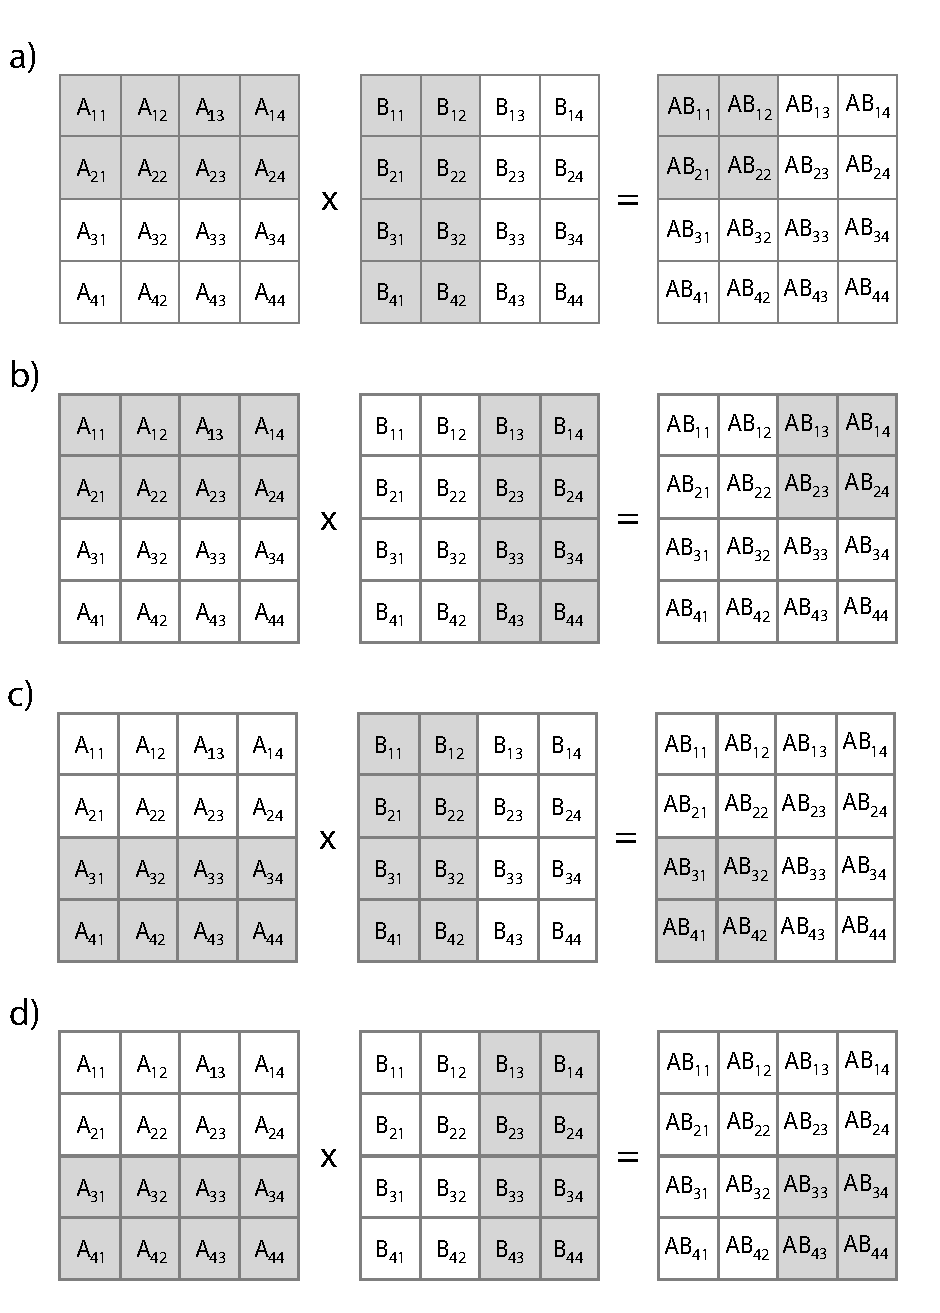
\includegraphics[width=  .85\textwidth]{images/blockmm}
\caption{ One possible blocked decomposition of the matrix multiplication of two $4 \times 4$ matrices. The entire $\mathbf{AB}$ product is decomposed into four matrix multiply operations operating on a $2 \times 4$ block of $\mathbf{A}$ and a $4 \times 2$ block of $\mathbf{B}$.}
\label{fig:blockmm}
\end{figure}

Figure \ref{fig:blockmm} provides the a description of the streaming architecture that we create. Our architecture has a variable \lstinline{BLOCK_SIZE} that indicates the number of rows that we take from the $\mathbf{A}$ matrix on each execution, the number of columns taken from the $\mathbf{B}$ matrix, and the \lstinline{BLOCK_SIZE} $\times$ \lstinline{BLOCK_SIZE} result matrix corresponding to the data that we compute each time for the $\mathbf{AB}$ matrix. 

The example in Figure \ref{fig:blockmm} uses a \lstinline{BLOCK_SIZE = 2}. Thus we take two rows from $\mathbf{A}$, and two columns from $\mathbf{B}$  on each execution of the streaming architecture that we define. The result of each call to the \lstinline{blockmatmul} function is a $2 \times 2$ matrix for the $\mathbf{AB}$ architecture.

Since we are dealing with $4 \times 4$ matrices in the example, we need to do this process four times. Each time we get a $2 \times 2$ set of results for the $\mathbf{AB}$ matrix. The figure shows a progression of the rows and columns that we send. In Figure \ref{fig:blockmm} a) we send the first two rows of $\mathbf{A}$ and the first two columns of $\mathbf{B}$. The function will compute a $2 \times 2$ matrix corresponding to the first two elements in the rows and columns of the resulting matrix $\mathbf{AB}$. 

In Figure \ref{fig:blockmm} b), we use again the first two rows of $\mathbf{A}$, but this time we send the last two columns of $\mathbf{B}$. We do not need to resend the data from the rows of $\mathbf{A}$ since they are the same as the previous data from the previous execution. And we get the results for the $2 \times 2$ matrix corresponding to the data in ``upper left'' corner of $\mathbf{AB}$. 

Figure \ref{fig:blockmm} c) sends different data for both the $\mathbf{A}$ and $\mathbf{B}$ matrices. This time we send the last two rows of $\mathbf{A}$ and the first two columns of $\mathbf{B}$. The results from this computation provide the ``lower left'' corner of the $\mathbf{AB}$ matrix.

The final execution of the streaming block matrix multiply, shown in Figure \ref{fig:blockmm} d), uses the same last two rows of the $\mathbf{A}$ matrix from the previous iteration. And it sends the last two columns of the $\mathbf{B}$ matrix. The result provides the elements in the ``lower right'' corner of the $\mathbf{AB}$ matrix. 

\begin{figure}
\lstinputlisting{examples/block_mm.h}
\caption{  The header file for the block matrix multiplication architecture. The file defines the data types used within the function, the key constants, and the \lstinline{blockmatmul} function interface.   }
\label{fig:block_mm_h}
\end{figure}

Before we show the code for the block matrix multiplication, we define some data types that we will use. Figure \ref{fig:block_mm_h} shows the header file for the project. We create a custom data type \lstinline{DTYPE} that specifies the type of data that we will multiply in the $\mathbf{A}$ and $\mathbf{B}$ matrices, and the corresponding $\mathbf{AB}$ matrix. This is currently set to an \lstinline{int} data type.

\begin{aside}
It is good coding practice to use a custom data type in your designs. This allows you to easily change the data type, and to have one source of information so that you do not have errors when changing the data type in the future design iterations. And it is quite common to change the data type over the course of the design. For example, first you may start out with a \lstinline{float} or \lstinline{double} type while you get a functionally correct design. This also provides a baseline for error since later you will likely change your design to use fixed point data type.  Fixed point data can reduce the number of resources, and increase the performance potentially at the cost of a reduction in the precision of the resulting data. You will likely try many different fixed point types until you find the right tradeoff between accuracy/error, performance, and resource usage.
\end{aside}

\lstinline{SIZE} determines the number of rows and columns in the matrices to be multiplied. We limit this to square matrices although handling arbitrary matrix sizes could be done by changing the code in a number of different places. We leave that as an exercise for the reader.

\begin{exercise}
Change the code to allow it to handle matrices of arbitrary size. 
\end{exercise}

The \lstinline{BLOCK_SIZE} variable defines the number of rows from $\mathbf{A}$ and the number of columns from $\mathbf{B}$ that we operate upon in each execution. This also defines how much data that we stream at one time into the function. The output data that we receive from the function at each execution is an \lstinline{BLOCK_SIZE} $\times$ \lstinline{BLOCK_SIZE} portion of the $\mathbf{AB}$ matrix. 

The \lstinline{blockvec} data type is used to transfer the \lstinline{BLOCK_SIZE} rows of $\mathbf{A}$ and columns of $\mathbf{B}$ to the function on each execution. The \lstinline{blockmat} data type is where we store the partial results for the $\mathbf{AB}$ matrix. 

Finally, the \lstinline{blockmat} data type is a structure consisting of an \lstinline{BLOCK_SIZE} $\times$ \lstinline{BLOCK_SIZE} array. This holds the resulting values from one execution of the \lstinline{matrmatmul} function. 

The function prototype itself takes the two inputs which are both of the type \lstinline{hls::stream<blockvec> &}. These are a sequence of \lstinline{blockvec} data. Remember that a \lstinline{blockvec} is a data type that consists of an array with \lstinline{BLOCK_SIZE} elements. 

The \lstinline{hls::stream<>} template class is one way in \VHLS of creating a FIFO data structure that works well in simulation and synthesis. The samples are sent in sequential order using the \lstinline{write()} function, and retrieved using the \lstinline{read()} function. This library was developed since streaming is a common methodology for passing data in hardware design, yet this same operation can be modeled in many different ways using the C programming language, for instance, by using arrays. In particular, it can be difficult for the \VHLS tool to infer streaming behaviors when dealing complex access patterns or multi-dimensional arrays. The built-in stream library enables the programmer to explicitly specify the order of stream accesses, avoiding any limitations of this inference. 

\begin{aside}
The \lstinline{hls::stream} class must always be passed by reference between functions, e.g., as we have done in the \lstinline{blockmatmul} function in Figure \ref{fig:block_mm}.
\end{aside}

\begin{figure}
\lstinputlisting[format=none]{examples/block_mm.cpp}
\caption{  The \lstinline{blockmatmul} function takes a \lstinline{BLOCK_SIZE} set of rows from $\mathbf{A}$ matrix, a \lstinline{BLOCK_SIZE} set of columns from the $\mathbf{B}$ matrix, and creates a \lstinline{BLOCK_SIZE} $\times$ \lstinline{BLOCK_SIZE} partial result for the $\mathbf{AB}$ matrix. The first part of the code (denoted by the label \lstinline{loadA}) stores the rows from $\mathbf{A}$ into a local memory, the second part in the nested \lstinline{partialsum for} performs the computation for the partial results, and the final part (with the \lstinline{writeoutput} label) takes these results and puts them the proper form to return from the function.}
\label{fig:block_mm}
\end{figure}

The code for executing one part of the streaming block matrix multiplication is shown in Figure \ref{fig:block_mm}. The code has three portions denoted by the labels \lstinline{loadA}, \lstinline{partialsum}, and \lstinline{writeoutput}. 

The first part of the code, denoted by the \lstinline{loadA} label, is only executed on certain conditions, more precisely when \lstinline{it % (SIZE/BLOCK_SIZE) == 0}. This is done to save some time in the cases when we can reuse the data from the $\mathbf{A}$ matrix from the previous execution of the function. 

Remember that in each execution of this \lstinline{blockmatmul} function we send \lstinline{BLOCK_SIZE} rows from the $\mathbf{A}$ matrix and \lstinline{BLOCK_SIZE} columns from the $\mathbf{B}$ matrix. We send multiple \lstinline{BLOCK_SIZE} of columns for each \lstinline{BLOCK_SIZE} of rows from $\mathbf{A}$. The variable \lstinline{it} keeps track of the number of times that we have called the \lstinline{blockmatmul} function. Thus, we do a check on each execution of the function to determine if we need to load the rows from $\mathbf{A}$. When we do not, this saves us some time. When it is executed, it simply pulls data from the \lstinline{Arows} stream and puts it into a static local two-dimensional matrix \lstinline{A[BLOCK_SIZE][SIZE]}. 

Fully understanding this code requires some explanation about the \lstinline{stream} class, and how we are using it. The \lstinline{stream} variable \lstinline{Arows} has elements of the type \lstinline{blockvec}. A \lstinline{blockvec} is a matrix of size \lstinline{BLOCK_SIZE}. We use this in the following manner; each element in the \lstinline{Arows} stream has an array that holds one element from each of the \lstinline{BLOCK_SIZE} rows of the $\mathbf{A}$ matrix. Thus, in each call the the \lstinline{blockmatmul} function, the \lstinline{Arows} stream will have \lstinline{SIZE} elements in it, each of those holding one of each of the \lstinline{BLOCK_SIZE} rows. The statement \lstinline{tempA = Arows.read()} takes one element from the \lstinline{Arows} stream. Then we load each of these elements into the appropriate index in the local \lstinline{A} matrix.

\begin{aside}
The \lstinline{stream} class overloads the \lstinline{<<} operator to be equivalent to the \lstinline{read()} function. Thus, the statements \lstinline{tempA = Arows.read()} and \lstinline{tempA << Arows} perform the same operation.
\end{aside}

The next part of the computation calculates the partial sums. This is the bulk of the computation in the \lstinline{blockmatmul} function. 

The \lstinline{Bcols} stream variable is utilized in a very similar manner to the \lstinline{Arows} variable. However, instead of storing rows of $\mathbf{A}$, it stores the data corresponding the columns of $\mathbf{B}$ that the current execution of the function is computing upon. Every call of the \lstinline{blockmatmul} function will provide new data for the columns of the $\mathbf{B}$ matrix. Thus, we do not need to conditionally load this data as we do with the $\mathbf{A}$ matrix. The function itself works in a very similar manner to that from the \lstinline{matmul} in Figure \ref{fig:matrixmultiplication_sw} except that we are only calculating \lstinline{BLOCK_SIZE} $\times$ \lstinline{BLOCK_SIZE} results from the $\mathbf{AB}$ matrix. Thus we only have to iterate across \lstinline{BLOCK_SIZE} rows of $\mathbf{A}$ and \lstinline{BLOCK_SIZE} columns of $\mathbf{B}$. But each row and column has \lstinline{SIZE} elements, hence the bounds on the outer \lstinline{for} loop. 

The final portion of the function moves the data from the local \lstinline{AB} array, which has dimensions of \lstinline{BLOCK_SIZE} $\times$ \lstinline{BLOCK_SIZE}; this holds the partial results of the $\mathbf{AB}$ output matrix. %The results are written into the \lstinline{out_temp} variable, which has the data type \lstinline{blockmat}. This data type is a \lstinline{BLOCK_SIZE} $\times$ \lstinline{BLOCK_SIZE} two dimension matrix. The \lstinline{out_temp} data is pushed into the \lstinline{ABpartial} stream in the statement \lstinline{ABpartial.write(out_temp);}

Of the three parts of the function, the middle part, which calculates the partial sum, requires the most computation. By inspecting the code, we can see that this part has three nested \lstinline{for} loops with a total of \lstinline{SIZE} $\times$ \lstinline{BLOCK_SIZE} $\times$ \lstinline{BLOCK_SIZE} iterations. The first part has \lstinline{SIZE} $\times$ \lstinline{BLOCK_SIZE} iterations; and the last part has \lstinline{BLOCK_SIZE} $\times$ \lstinline{BLOCK_SIZE} iterations. Thus, we should focus our optimizations on the middle part, i.e., the \lstinline{partialsum} nested \lstinline{for} loops.

The common starting point for optimizations of nested \lstinline{for} loops is to pipeline the innermost \lstinline{for} loop. Then, if that does not require too many resources, the designer can move the \lstinline{pipeline} directive into higher level \lstinline{for} loops. Whether the resulting design consume too many resource depends upon the specified \lstinline{BLOCK_SIZE}; if this is small, then it is likely worth moving the \lstinline{pipeline} directive. It may even be worthwhile to move it inside the outermost \lstinline{for} loop. This will unroll the two inner \lstinline{for} loops and thus very likely increase the resource usage by a substantial amount. However, it will increase the performance.

\begin{exercise}
How does changing the \lstinline{BLOCK_SIZE} effect the performance and resource usage? How about changing the \lstinline{SIZE} constant? How does moving the \lstinline{pipeline} directive across the three different nested \lstinline{for} loops in the \lstinline{partialsum} portion of the function change the performance and resource usage?
\end{exercise}

The \lstinline{dataflow} directive at the start of the function creates a pipeline across the portions of the function, i.e., the \lstinline{loadA for} loop, the \lstinline{partialsum} nested \lstinline{for} loop, and the \lstinline{writeoutput for} loop. Using this directive will decrease the interval of the \lstinline{blockmatmul} function. However, this is limited by the largest interval of all three of the portions of the code. That is, the maximum interval for the \lstinline{blockmatmul} function -- let us call it interval(\lstinline{blockmatmul}) -- is greater than or equal to the the interval of the three parts which are defined as interval(\lstinline{loadA}), interval(\lstinline{partialsum}), and interval(\lstinline{writeoutput}). More formally, 

\begin{align}
\label{eq:interval}
interval(\texttt{blockmatmul}) \ge \max(&interval(\texttt{loadA}), interval(\texttt{partialsum}), \nonumber \\
 & interval(\texttt{writeoutput}))
 \end{align}

We need to keep Equation \ref{eq:interval} in mind as we optimize the \lstinline{blockmatmul} function. For example, assume that interval(\lstinline{partialsum}) is much larger than the other two portions of the function. Any performance optimizations that minimize interval(\lstinline{loadA}) and interval(\lstinline{writeoutput}) are useless since the function interval, i.e., interval(\lstinline{blockmatmul}) would not decrease. Thus, the designer should focus any performance optimization effort to decrease interval(\lstinline{partialsum}), i.e., target performance optimizations on those three nested \lstinline{for} loops. 

It is important to note that this only applies to performance optimizations. The designer can (and should) optimize the resource usage of these other two parts. In fact, they are ripe for such optimizations since reducing the resource usage often increases the interval and/or latency. In this case, it is ok to increase the interval as it will not effect the overall performance of the \lstinline{blockmatmul} function. In fact, the ideal case is to optimize all three parts of the function such that they all have the same interval, assuming that we can easily tradeoff between the interval and resource usage (which is not always the case). 

The testbench for the \lstinline{blockmatmul} function is shown in Figures \ref{fig:block_mm_init} and \ref{fig:block_mm_final}. We split it across two figures to make it more readable since it is a longer piece of code. Up until this point, we have not shown the testbenches. We show this testbench for several reasons. First, it provides insight into how the \lstinline{blockmatmul} function works. In particular, it partitions the input matrices into blocks and feeds them into the \lstinline{blockmatmul} function in a block by block manner. Second, it gives a complex usage scenario for using \lstinline{stream} template for simulation. Finally, it gives the reader an idea about how to properly design testbenches.

The \lstinline{matmatmul_sw} function is a simple three \lstinline{for} loop implementation of matrix multiplication. It takes two two-dimensional matrices as inputs, and outputs a single two-dimensional matrix. It is very similar to what we have seen in the \lstinline{matrixmul} function in Figure \ref{fig:matrixmultiplication_sw}. We use this to compare our results from the blocked matrix multiplication hardware version.

Let us focus on the first half of the testbench shown in Figure \ref{fig:block_mm_init}. The beginning block of code initializes variables of the rest of the function. The variable \lstinline{fail} keeps track of whether the matrix multiplication was done correctly. We will check this later in the function. The variables \lstinline{strm_matrix1} and \lstinline{strm_matrix2} are \lstinline{hls:stream<>} variables that hold the rows and columns of the $\mathbf{A}$ and $\mathbf{B}$ matrices, respectively. Each element of these \lstinline{stream} variables is a \lstinline{<blockvec>}. Referring back at the \lstinline{block_mm.h} file in Figure \ref{fig:block_mm_h}, we recall that a \lstinline{blockvec} is defined as an array of data; we will use each \lstinline{blockvec} to store one row or column of data. 

\begin{aside}
The \lstinline{stream} variable resides in the \lstinline{hls} namespace. Thus, we can use that namespace and forgo the \lstinline{hls::stream} and instead simply use \lstinline{stream}. However, the preferred usage is to keep the \lstinline{hls::} in front of the \lstinline{stream} to insure code readers that the stream is relevant to \VHLS and not C construct from another library. Also, it avoids having to deal with any potential conflicts that may occur by introducing a new namespace.
\end{aside}

The next definitions in this beginning block of code are the variables \lstinline{strm_matrix1_element} and \lstinline{strm_matrix2_element}. These two variables are used as placeholders to populate each \lstinline{blockvec} variable that we write into the \lstinline{strm_matrix1} and \lstinline{strm_matrix2} stream variables. The \lstinline{block_out} variable is used to store the output results from the \lstinline{blockmatmul} function. Note that this variable uses the data type \lstinline{blockmat} which is a two-dimensional array of \lstinline{BLOCK_SIZE} $\times$ \lstinline{BLOCK_SIZE} as defined in the \lstinline{block_mm.h} header file (see Figure \ref{fig:block_mm_h}). The final definitions are \lstinline{A},  \lstinline{B},  \lstinline{matrix_swout},  and\lstinline{matrix_hwout}. These are all \lstinline{SIZE} $\times$ \lstinline{SIZE} two-dimensional arrays with the \lstinline{DTYPE} data type. 

\begin{aside}
You can name the streams using an initializer. This is good practice as it gives better error messages. Without the name, the error message provides a generic reference to the stream with the data type. If you have multiple stream declarations with the same data type, then you will have to figure out which stream the error is referring to. Naming the stream variable is done by giving the variable an argument which is the name, e.g., \lstinline{hls::stream<blockvec> strm_matrix1("strm_matrix1");}.
\end{aside}

The next set of nested \lstinline{initmatrices for} loops sets the values of the four two-dimensional arrays \lstinline{A}, \lstinline{B}, \lstinline{matrix_swout}, and \lstinline{matrix_hwout}. The variables \lstinline{A} and \lstinline{B} are input matrices. These are initialized to a random value between [0, 512). We picked the number 512 for no particular reason other than it can fit any 9 bit value. Keep in mind that while the \lstinline{DTYPE} is set as an \lstinline{int}, and thus has significantly more range than [0,512), we often move to fixed point values with much smaller ranges later in the design optimization process. The \lstinline{matrix_swout} and \lstinline{matrix_hwout} are both initialized to $0$. These are filled in later by calls to the functions \lstinline{matmatmul_sw} and \lstinline{blockmatmul}.

\begin{figure}
\lstinputlisting{examples/blockmatmul_test_init.cpp}
\caption{  The first part of the testbench for block matrix multiplication. The function is split across two figures since it is too long to display on one page. The rest of the testbench is in Figure \ref{fig:block_mm_final}. This has a ``software'' version of matrix multiplication, and variable declarations and initializations. }
\label{fig:block_mm_init}
\end{figure}

The second part of the testbench is continued in Figure \ref{fig:block_mm_final}. This has the last portion of the code from the \lstinline{main} function. 

\begin{figure}
\lstinputlisting[format=none]{examples/blockmatmul_test.cpp}
\caption{  The second portion of the block matrix multiply testbench. The first part is shown in Figure \ref{fig:block_mm_init}. This shows the computation required to stream the data to the \lstinline{blockmatmul} function, and the code that tests that this function matches a simpler three \lstinline{for} loop implementation. }
\label{fig:block_mm_final}
\end{figure}

The first part of this figure has a complex set of nested \lstinline{for} loops. The overall goal of the computation in these \lstinline{for} loops is to set up the data from the input matrices $\mathbf{A}$ and $\mathbf{B}$ so that it can be streamed to the \lstinline{blockmatmul} function. Then the results of the \lstinline{blockmatmul} function are stored in the \lstinline{matrix_hwout} array. 

The outer two \lstinline{for} loops are used to step across the input arrays in a blocked manner. You can see that these both iterate by a step of \lstinline{BLOCK_SIZE}. The next two \lstinline{for} loops write rows from $\mathbf{A}$ into \lstinline{strm_matrix1_element} and the columns from $\mathbf{B}$ into \lstinline{strm_matrix2_element}. It does this in an element by element fashion by using the variable \lstinline{k} to access the individual values from the rows (columns) and write these into the one dimensional array for each of these ``elements''. Remember that both \lstinline{strm_matrix1_element} and \lstinline{strm_matrix2_element} have the datatype \lstinline{blockvec}, which is a one dimensional array of size \lstinline{BLOCK_SIZE}. It is meant to hold \lstinline{BLOCK_SIZE} elements from each row or column. The inner \lstinline{for} loop iterates \lstinline{BLOCK_SIZE} times. The \lstinline{strm_matrix1} and \lstinline{strm_matrix2} stream variables are written to \lstinline{SIZE} times. That means that has a buffer of the entire row (or column) and each element in the buffer holds \lstinline{BLOCK_SIZE} values. 

\begin{aside}
The \lstinline{stream} class overloads the \lstinline{>>} operator to be equivalent to the \lstinline{write(data)} function. This is similar to overloading the \lstinline{read()} function to the \lstinline{<<} operator. Thus, the statements \lstinline{strm_matrix1.write(strm_matrix1_element)} and \lstinline{strm_matrix1_element >> strm_matrix1} perform the same operation.
\end{aside}

The final part of this portion of the code to highlight is the \lstinline{if} statements. These are correspond to the values $\mathbf{A}$ matrix. Essentially, these are there so that we do not constantly write the same values to \lstinline{strm_matrix1}. Recall that the values from the $\mathbf{A}$ matrix are used across several calls to the \lstinline{blockmatmul} function. See Figure \ref{fig:blockmm} for a discussion on this. These \lstinline{if} statements are placed there to highlight the fact that you should not continually write the same data over and over. This is important because the internal code of the \lstinline{blockmatmul} only does a read of this data when it is necessary. So if we continued to write this consistently, the code would not function correctly do to the fact that this stream is written to more than it is read from.

Now that the input data, the testbench calls the \lstinline{blockmatmul} function. After the function call, it receives the partial computed results in the \lstinline{block_out} variable. The next two \lstinline{for} loops but these results into the appropriate locations in the \lstinline{matrix_hwout} array. 

After this complex set of \lstinline{for} loops, the block matrix multiplication is complete. And the testbench continues to insure that the code is written correctly. It does this by comparing the results from the multiple calls to the \lstinline{blockmatmul} function to results that were computed in the \lstinline{matmatmul_sw}, which is a much simpler version of matrix matrix multiplication. After this function call, the testbench iterates through both two-dimensional matrices \lstinline{matrix_hwout} and \lstinline{matrix_swout} and makes sure that all of the elements are equivalent. If there is one or more element that is not equal, it sets the \lstinline{fail} flag equal to 1. The testbench completes by printing out \lstinline{failed} or \lstinline{passed}.

\begin{aside}
It is important that note that you cannot directly compare the performance of the function \lstinline{blockmatmul} with that of code for matrix multiplication, such as the code in Figure \ref{fig:matrixmultiplication_sw}. This is because it takes multiple calls to the \lstinline{blockmatmul} function in order to perform the entire matrix multiplication. It is important to always compare apples to apples.

\begin{exercise}
Derive a function to determine the number of times that \lstinline{blockmatmul} must be called in order to complete the entire matrix multiplication. This function should be generic, e.g., it should not be assume a specific value of \lstinline{BLOCK_SIZE} or size of the matrix (i.e., \lstinline{SIZE}).
\end{exercise}

\begin{exercise}
Compare the resource usage of block matrix multiplication versus matrix multiplication. How do the resources change as the size of the matrices increases? Does the block size play a role in the resource usage? What are the general trends, if any?
\end{exercise}

\begin{exercise}
Compare the performance of block matrix multiplication versus matrix multiplication. How does the performance change as the size of the matrices increases? Does the block size play a role in the performance? Pick two architectures with similar resource usage. How does the performance for those architectures compare?
\end{exercise}

\end{aside}

\section{Conclusion}

Block matrix multiplication provides a different way to compute matrix multiplication. It computes partial results of the result matrix by streaming a subset of the input matrices to a function. This function is then computed multiple times in order to complete the entire matrix multiplication computation. 


